\subsubsection{rendering.tick}
    Enthält die Klassen und Funktionalität um \textit{Tick}s auf den Scenegraph der JMonkeyEngine anzuwenden.\par

    \begin{figure}[htbp]
        \centering
        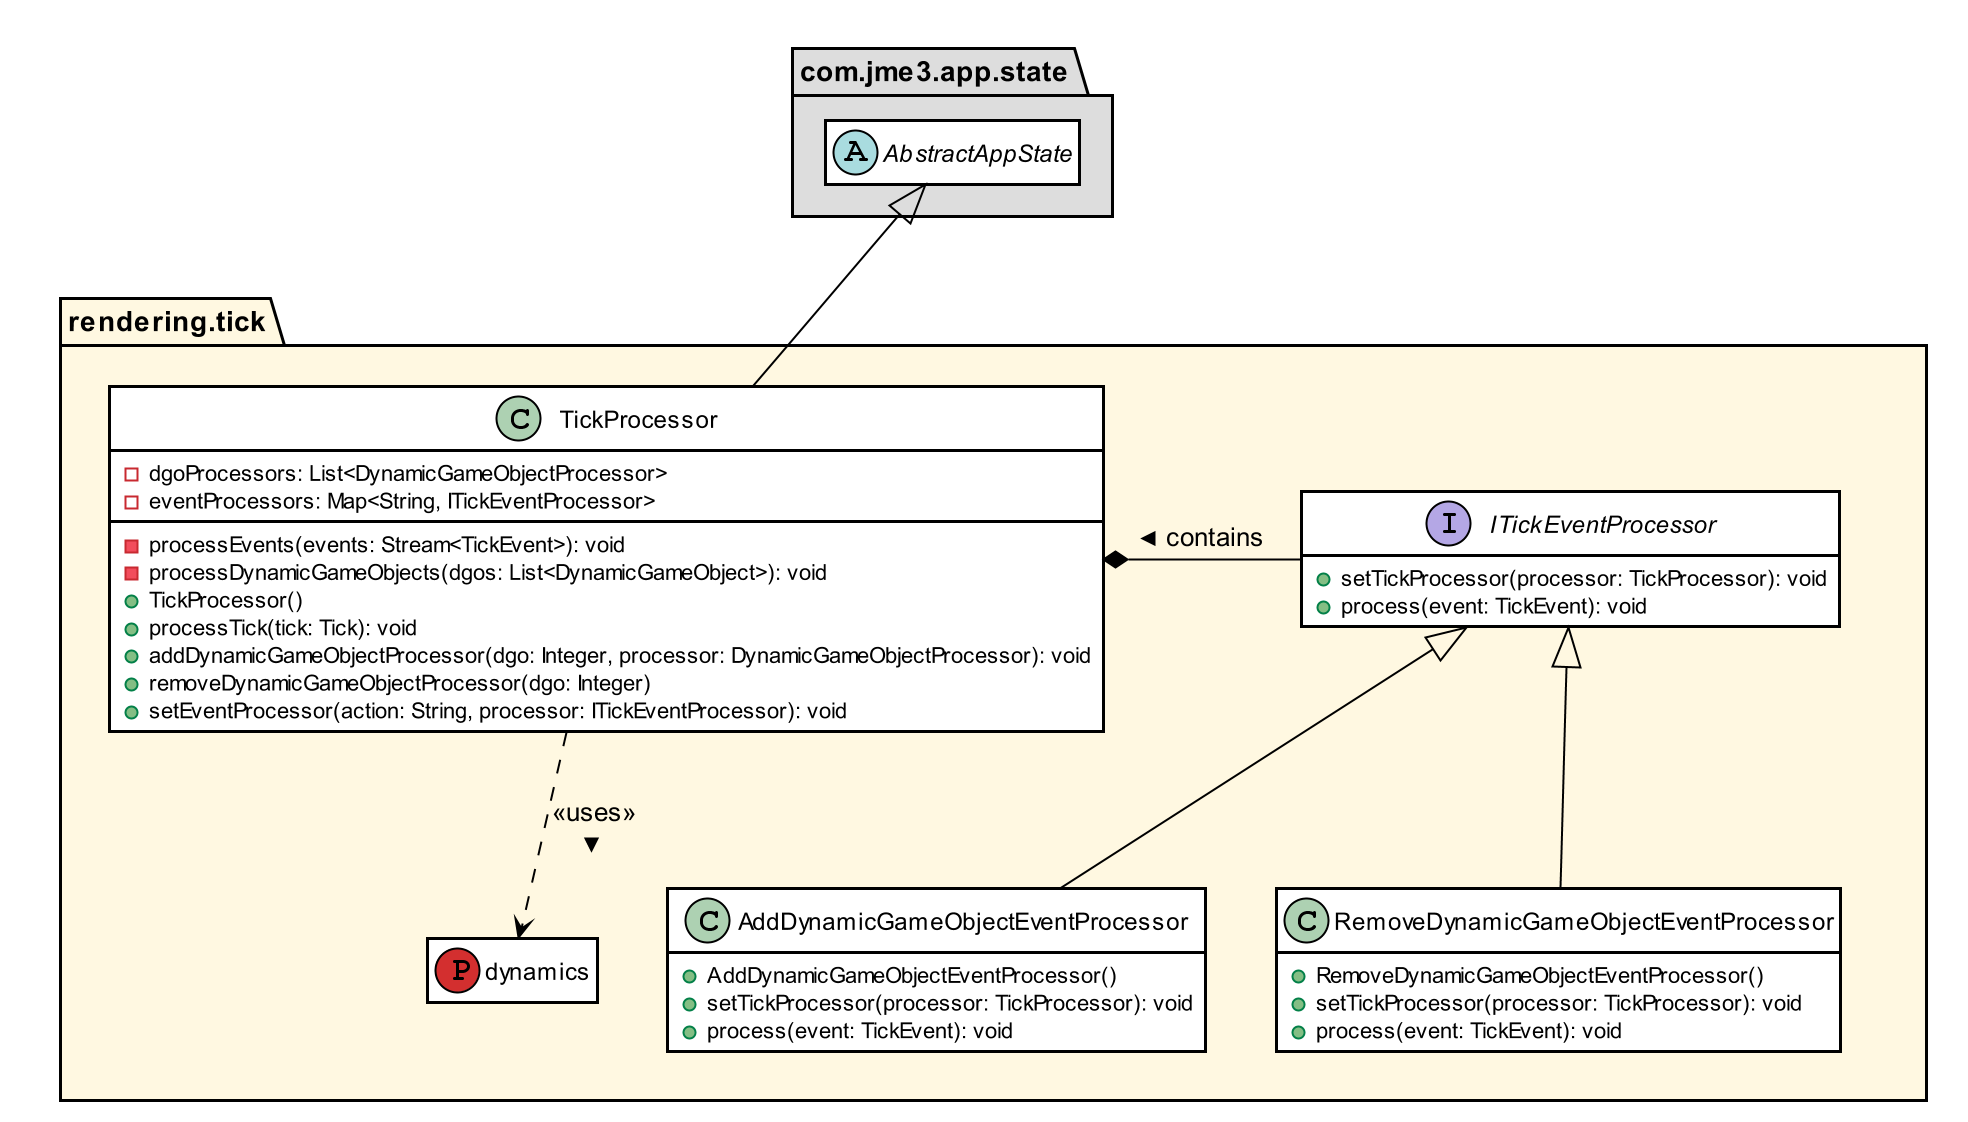
\includegraphics[width=\linewidth]{Interface/render-tick.png}
        \caption{rendering.tick Klassen-Diagram}
    \end{figure}

        \paragraph{\underline{TickProcessor}} \mbox{}\\
        \\
            Verarbeitet \textit{Tick}s indem er die in diesem enthaltenen \textit{DynamicGameObject}s an
            \textit{DynamicGameObjectProcessor}s weiterleitet und \textit{TickEvent}s mit den zugehörigen \textit{ITickEventProcessor}s bearbeitet.\par
                    
            \textbf{Attribute}
            \begin{itemize}
                \item \textit{- List<DynamicGameObjectProcessor> dgoProcessors}
                    \begin{leftbar}[0.9\linewidth]
                        Enthält alle \textit{DynamicGameObjectProcessor}s welche aktuell bekannt sind.
                    \end{leftbar}
                \item \textit{- Map<String, ITickEventProcessor> eventProcessors}
                    \begin{leftbar}[0.9\linewidth]
                        Enthält für jede bekannte Aktion eines \textit{TickEvent}s einen \textit{ITickEventProcessor}.
                    \end{leftbar}
            \end{itemize}

            \textbf{Methoden}
            \begin{itemize}
                \item  \textit{+ TickProcessor()}
                    \begin{leftbar}[0.9\linewidth]
                        Erstellt einen \textit{TickProcessor} und initialisiert dgoProcessors als leere List und eventProcessors als leere Map.
                    \end{leftbar}

                \pagebreak
                \item \textit{+ processTick(Tick tick): void}
                    \begin{leftbar}[0.9\linewidth]
                        Zunächst die \textit{TickEvent}s im gegebenen \textit{Tick} und leitet anschließend die \textit{DynamicGameObject}s
                        an die entsprechenden \textit{DynamicGameObjectProcessor}s weiter.\\
                        \textbf{@param tick} der zu bearbeitende \textit{Tick}.
                    \end{leftbar}
                \item \textit{+ addDynamicGameObjectProcessor(Integer dgo, DynamicGameObjectProcessor processor): void}
                    \begin{leftbar}[0.9\linewidth]
                        Fügt einen neuen \textit{DynamicGameObjectProcessor} für das \textit{DynamicGameObject} mit dem gegebenen index
                        zu diesem \textit{TickProcessor} hinzu.\\
                        \textbf{@param dgo} der index des \textit{DynamicGameObjects}, für welches der \textit{DynamicGameObjectProcessor} hinzugefügt werden soll.\\
                        \textbf{@param processor} der \textit{DynamicGameObjectProcessor}, welcher hinzugefügt werden soll.
                    \end{leftbar}
                \item \textit{+ removeDynamicGameObjectProcessor(int dgo): void}
                    \begin{leftbar}[0.9\linewidth]
                        Entfernt den \textit{DynamicGameObjectProcessor} des \textit{DynamicGameObject}s mit dem gegebenen index.\\
                        \textbf{@param dgo} der index des \textit{DynamicGameObjects}, dessen \textit{DynamicGameObjectProcessor} entfernt werden soll.
                    \end{leftbar}
                \item \textit{+ setEventProcessor(String action, ITickEventProcessor processor): void}
                    \begin{leftbar}[0.9\linewidth]
                        Setzt den \textit{ITickEventProcessor} welcher für \textit{TickEvent}s mit der gegebenen Aktion verwendet werden soll.\\
                        \textbf{@param action} die Aktion, für welche der \textit{ITickEventProcessor} gesetzt werden soll.\\
                        \textbf{@param processor} der \textit{ITickEventProcessor}, welcher gesetzt werden soll.
                    \end{leftbar}
            \end{itemize}

        \paragraph{\underline{ITickEventProcessor}} \mbox{}\\
        \\
            Interface welches die Funktionalität, welche benötigt ist um ein \textit{TickEvent} für den \textit{TickProcessor} zu verarbeiten, festlegt.\par

            \textbf{Methoden}					
            \begin{itemize}
                \item  \textit{+ setTickProcessor(TickProcessor processor): void}
                    \begin{leftbar}[0.9\linewidth]
                        Setzt den \textit{TickProcessor}, welcher diesen \textit{ITickEventProcessor} verwenden wird, fest.\\
                        \textbf{@param processor} der \textit{TickProcessor}, welcher diesen \textit{ITickEventProcessor} verwendet.
                    \end{leftbar}

                \pagebreak

                \item  \textit{+ process(TickEvent event): void}
                    \begin{leftbar}[0.9\linewidth]
                        Wird aufgerufen, sobald ein \textit{TickEvent} mit der Aktion, für die dieser \textit{ITickEventProcessor} registriert wurde, auftritt.\\
                        \textbf{@param event} das zu verarbeitende \textit{TickEvent}.
                    \end{leftbar}
            \end{itemize}

        \paragraph{\underline{AddDynamicGameObjectEventProcessor}} \mbox{}\\
        \\
        \textit{ITickEventProcessor} zur Bearbeitung eines \textit{TickEvent}s, welches auftritt, wenn ein neues \textit{DynamicGameObject} hinzugefügt wurde.\par

            \textbf{Attribute}
            \begin{itemize}
                \item  \textit{- TickProcessor tickProcessor}
                    \begin{leftbar}[0.9\linewidth]
                        Der \textit{TickProcessor}, welcher diesen \textit{ITickEventProcessor} verwendet.
                    \end{leftbar}
            \end{itemize}
            \textbf{Methoden}					
            \begin{itemize}
                \item  \textit{+ AddDynamicGameObjectEventProcessor()}
                    \begin{leftbar}[0.9\linewidth]
                        Erstellt einen neuen \textit{AddDynamicGameObjectEventProcessor}.
                    \end{leftbar}
                \item  \textit{+ setTickProcessor(TickProcessor processor): void}
                    \begin{leftbar}[0.9\linewidth]
                        Siehe \textit{ITickEventProcessor.setTickProcessor()}.
                    \end{leftbar}
                \item  \textit{+ process(TickEvent event): void}
                    \begin{leftbar}[0.9\linewidth]
                        Siehe \textit{ITickEventProcessor.process()}.
                    \end{leftbar}
            \end{itemize}

        \pagebreak
        \paragraph{\underline{RemoveDynamicGameObjectEventProcessor}} \mbox{}\\
        \\
        \textit{ITickEventProcessor} zur Bearbeitung eines \textit{TickEvent}s, welches auftritt, wenn \textit{DynamicGameObject} entfernt wurde.\par

            \textbf{Attribute}
            \begin{itemize}
                \item  \textit{- TickProcessor tickProcessor}
                    \begin{leftbar}[0.9\linewidth]
                        Der \textit{TickProcessor}, welcher diesen \textit{ITickEventProcessor} verwendet.
                    \end{leftbar}
            \end{itemize}
            \textbf{Methoden}					
            \begin{itemize}
                \item  \textit{+ RemoveDynamicGameObjectEventProcessor()}
                    \begin{leftbar}[0.9\linewidth]
                        Erstellt einen neuen \textit{RemoveDynamicGameObjectEventProcessor}.
                    \end{leftbar}
                \item \textit{+ setTickProcessor(TickProcessor processor): void}
                    \begin{leftbar}[0.9\linewidth]
                        Siehe \textit{ITickEventProcessor.setTickProcessor()}.
                    \end{leftbar}
                \item  \textit{+ process(TickEvent event): void}
                    \begin{leftbar}[0.9\linewidth]
                        Siehe \textit{ITickEventProcessor.process()}.
                    \end{leftbar}
            \end{itemize}